%!TEX root = cahier_charges_afnor.tex
\section{Cadre de réponse}

\subsection{Options et variantes proposées non retenues au cahier des charges}

Nous souhaitions au départ proposer une architecture modulaire pour le stockage des données afin d'implanter la sérialisation.

Nous souhaitions proposer messagerie instantanée et courriers type E-mail, puis un regroupement de ces fonctionnalités nous a semblé favorable.

L'utilisation du \emph{framework} Qt Jambi pour l'interface graphique a été rapidement écarté pour permettre l'utilisation de JWS.

\subsection{Mesures prises pour respecter les contraintes}

\begin{figure}[thbp]
	\centering
		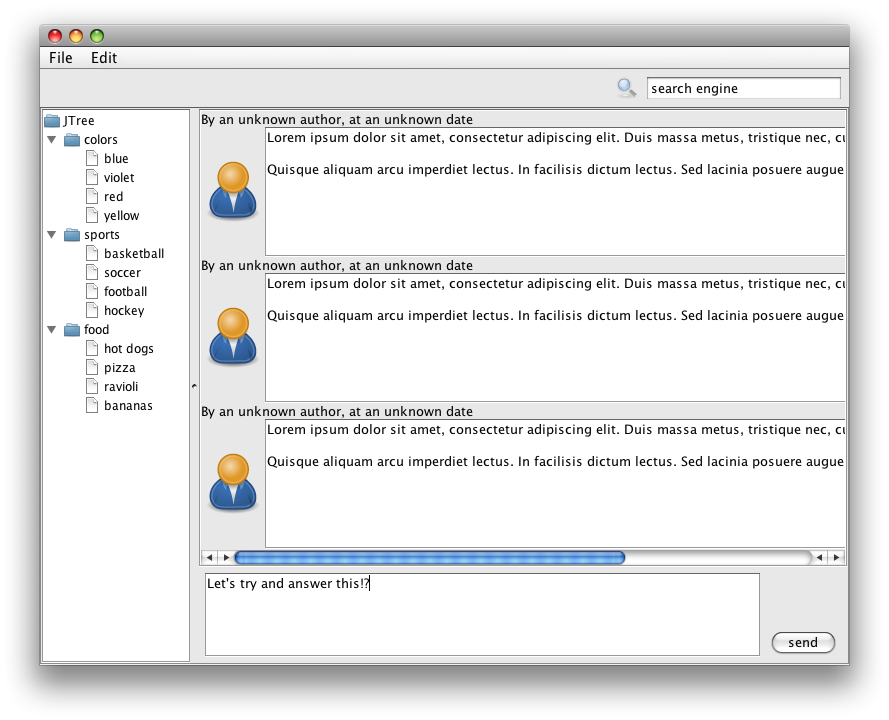
\includegraphics[width=15cm]{proto_client.png}
	\caption{Prototype d'interface}
	\label{fig:proto}
\end{figure}

Le choix d'un client lourd a rapidement écarté l'utilisation de thèmes CSS puisque JWebPanel est encore instable. Un prototype de l'interface permettant d'en percevoir la conception générale est proposé figure~\ref{fig:proto}.

\subsection{Outils d’installation, de maintenance}

Le produit sera livré sous forme d'archives JAR contenant la librairie et les programmes témoins.

Les clients pourront utiliser la technologie Java Web Start pour distribuer l'application à tous leurs utilisateurs sans l'intervention des administrateurs.

La documentation sera distribuée sous forme d'archive (utilisation de javadoc) ainsi que d'une vidéo de démonstration du produit (\emph{screencast}).

\subsection{Perspectives d’évolution technologique}

Le produit pourra, plus tard, évoluer vers une version plus complète en ajoutant, par exemple, une gestion des événements ou le suivi des versions des modèles.
Il pourra aussi être doté d'une persistance de donnée abstraite de tout éditeur de serveur SQL au travers d'Hibernate.
